\subsection{Wechselwirkung ionisierender Strahlung mit Materie}
In dem Versuch ist die Wechselwirkung von $\gamma$-Quanten mit Materie relevant.
\subsubsection{Compton-Effekt} 
Beim Compton-Effekt streut ein Photon an einem Teilchen (siehe Abbildung \ref{fig:compton}). Dabei wird ein gewisser Impuls vom Photon auf das Teilchen übertragen. Abhängig von Ablenkwinkel $\phi$ des gestreuten Photons lässt sich aus der (Vierer-)Impulserhaltung die Wellenlänge des gestreuten Photons zu
\begin{align*}
  \lambda-\lambda_0=\frac{h}{mc}(1-\cos \phi)
\end{align*} 
berechnen. $h$ und $c$ sind dabei das Plancksche Wirkungsquantum und die Lichtgeschwindigkeit. $m$ ist die Masse des Teilchens. Der Ausdruck für die Wellenlängenverschiebung gilt in dem Bezugssystem, in dem das Teilchen zunächst ruht.
\begin{figure}[h]
  \centering
  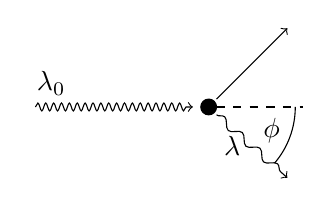
\begin{tikzpicture}[photon1/.style={decorate,decoration={snake, segment length=1mm, amplitude=0.5mm, post length=0.5mm}},photon2/.style={decorate,decoration={snake, segment length=3mm, amplitude=0.5mm, post length=0.5mm}}]
    \draw [->,photon1] (0,2)--(2,2);
    \draw [fill=black] (2.2,2) circle (0.1);
    \draw [->] (2.3,2.1)--(3.2,3);
    \draw [->,photon2] (2.3,1.9)--(3.2,1.1);
    \draw [dashed] (2.3,2)--(3.4,2);
    \draw (0.2,2.3) node {$\lambda_0$}; 
    \draw (2.5,1.5) node {$\lambda$};
    \draw (3.3,2) arc (0:-40.5:1.1);
    \draw (3,1.7) node {$\phi$};
  \end{tikzpicture}
  \caption{Compton-Effekt}
  \label{fig:compton}
\end{figure}

\subsubsection{Photoeffekt}
Beim Photoeffekt wird die Energie eines einfallenden Photons von einem Hüllenelektron eines Atoms absorbiert. Dadurch wird das Elektron ionisiert. Die kinetische Energie des Elektrons entspricht dann der ursprünglichen Energie des Photons abzüglich der Bindungsenergie des Elektrons.

\subsubsection{Paarbildung}
Bei der Paarbildung erzeugt ein energiereiches Photon ein Elektron-Positron-Paar. Die überschüssige Energie geht dabei in die kinetische Energie der erzeugten Teilchen. Ein Photon alleine kann noch nicht die Paarbildung auslösen. Es ist die Anwesenheit eines Atomkerns, eines Elektrons oder eines weiteren energiereichen Photons notwendig. 

\subsection{Szintillationszähler}
Ein Szintillator weist ionisierende Teilchen nach. Die Teilchen regen die Atome im Szintillationsmaterial an. Nach einer mittleren Anregungsdauer fällt das Atom zurück in den Grundzustand und emittiert dabei ein Photon der entsprechenden Wellenlänge. Dieses Photon kann nun auch wieder weitere Atome anregen und es kommt zu einer Art Random-Walk. Um diesen zu unterbrechen, wird das Szintillationsmaterial schwach mit wellenlängenverschiebenden Molekülen dotiert. Trifft ein Photon auf ein solches, wird das Licht zu langwelligerem Licht umgewandelt. Dieses kann nicht vom Szintillator absorbiert werden und somit über einen Lichtleiter zu einer Photodiode gelangen. Diese erzeugt eine messbare elektrische Spannung. Der Prozess ist in Abbildung \ref{fig:szintillator} schematisch skizziert.

\begin{figure}[h]
  \centering
  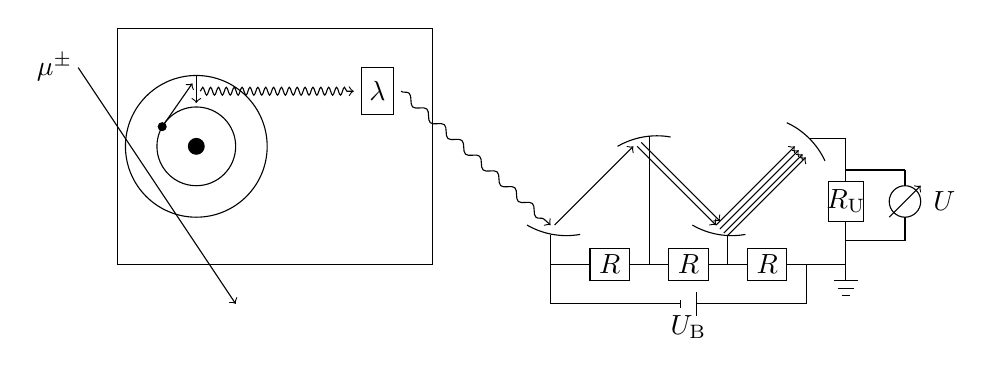
\begin{tikzpicture}[photon1/.style={decorate,decoration={snake, segment length=1mm, amplitude=0.5mm, post length=0.5mm}},photon2/.style={decorate,decoration={snake, segment length=3mm, amplitude=0.5mm, post length=0.5mm}}]
    \draw (0,0) rectangle (4,3);
    \draw [->] (-0.5,2.5)--(1.5,-0.5);
    \draw (-0.8,2.5) node {$\mu^{\pm}$};
    \draw (1,1.5) circle (0.9);
    \draw (1,1.5) circle (0.5);
    \draw [fill=black] (1,1.5) circle (0.1);
    \draw [fill=black] (1-0.5*1.732/2,1.5+1/4) circle (0.05);
    \draw [->] (1-0.5*1.732/2,1.5+1/4)--(0.95,2.3);
    \draw [->] (1,2.4) -- (1,2.05);
    \draw [->,photon1] (1.05,2.2) -- (3,2.2);
    \draw (3.1,1.9) rectangle (3.5,2.5);
    \draw (3.3,2.2) node {$\lambda$};
    \draw [->,photon2] (3.6,2.2)-- (5.5,0.5);
    \draw (5.2,0.5) arc (-120:-80:1);
    \draw [->] (5.55,0.5) -- (6.55,1.5);
    \draw (6.35,1.5) arc (120:80:1);
    \draw [->] (6.6,1.5) -- (7.6,0.5);
    \draw [->] (6.65,1.55) -- (7.65,0.55);
    \draw (7.3,0.5) arc (-120:-80:1);
    \draw [->] (7.65,0.45) -- (8.65,1.45);
    \draw [->] (7.6,0.5) -- (8.6,1.5);
    \draw [->] (7.7,0.4) -- (8.7,1.4);
    \draw [->] (7.74,0.36) -- (8.74,1.36);
    \draw (8.5,1.8) arc (65:25:1);
    \draw (9,0)--(8.5,0);
    \draw (8.75,0)--(8.75,-0.5)--(7.35,-0.5);
    \draw (7.15,-0.5)--(5.5,-0.5)--(5.5,0);
    \draw (8.5,0.2) rectangle (8,-0.2);
    \draw (8.25,0) node {$R$};
    \draw (8,0) -- (7.5,0);
    \draw (7.5,0.2) rectangle (7,-0.2);
    \draw (7.25,0) node {$R$};
    \draw (7,0) -- (6.5,0);
    \draw (7.75,0)--(7.75,0.375);
    \draw (6.75,0)--(6.75,1.635);
    \draw (6.5,0.2) rectangle (6,-0.2);
    \draw (6.25,0) node {$R$};
    \draw (6,0)--(5.5,0)--(5.5,0.375);
    \draw (7.35,-0.65)--(7.35,-0.35);
    \draw (7.15,-0.55)--(7.15,-0.45);
    \draw (7.25,-0.8) node {$U_\mathrm{B}$};
    \draw (9,0)--(9.25,0)--(9.25,0.55);
    \draw (9.03,0.55) rectangle (9.47,1.05);
    \draw (9.25,0.8) node {$R_\mathrm{U}$};
    \draw (9.25,1.05)--(9.25,1.6)--(8.8,1.6);
    \draw (9.25,0)--(9.25,-0.2);
    \draw (9.1,-0.2)--(9.4,-0.2);
    \draw (9.15,-0.3)--(9.35,-0.3);
    \draw (9.2,-0.4)--(9.3,-0.4);
    \draw (9.25,0.3)--(10,0.3);
    \draw (9.25,1.2)--(10,1.2);
    \draw (10,0.8) circle (0.2);
    \draw (10,0.3)--(10,0.6);
    \draw (10,1.2)--(10,1);
    \draw [->] (9.8,0.6)--(10.2,1);
    \draw (10.5,0.8) node {$U$};
  \end{tikzpicture}
  \caption{Signalerzeugung im Szintillator}
  \label{fig:szintillator}
\end{figure}

\subsection{Diskriminator und Koinzidenzmodul}
Für die Zählung der Myonen aus der kosmischen Strahlung werden die analogen Signale der Szintillatoren in digitale Signale umgewandelt. Dazu werden Diskriminatoren verwendet. Gibt der Szintillator ein Signal über der einstellbaren Schwellenspannung $\delta U$ an den Diskriminator, gibt dieser eine logische 1 in Form eines Rechteckpulses aus. Die Dauer $\delta t$ dieses Rechteckpulses ist ebenfalls einstellbar. Bei zu kleinem $\delta t$ kann ein einzelner Puls doppelt gezählt werden. Bei zu großem $\delta t$ hingegen kann ein Puls eines neuen Myons übersehen werden. Beide Fälle sowie der optimale Fall sind in Abbildung \ref{fig:diskriminator} zu sehen.

\begin{figure}[h]
  \centering
  \begin{tikzpicture}
    \draw [->] (0,0)--(0,4.5) node [left] {$U$};
    \draw [->] (0,0)--(10.5,0) node [right] {$t$};
    \draw[domain=0:10,smooth,variable=\x,samples=200] plot ({\x},{3*exp(-2*(\x-1)^2)+3.5*exp(-0.5*(\x-1-4)^2)+4*exp(-40*(\x-2-7)^2)+4*exp(-40*(\x-2-7.5)^2)});
    \draw [dashed] (0,0)--(0.698,0)--(0.698,2.5)--(1.698,2.5)--(1.698,0)--(4.18,0)--(4.18,2.5)--(5.18,2.5)--(5.18,0);
    \draw [dashed] (5.18,2.5)--(6.18,2.5)--(6.18,0)--(8.892,0)--(8.892,2.5)--(9.892,2.5)--(9.892,0);
    \draw [<->] (11.5,2.5)--(12,2.5) node [right] {$1$};
    \draw [<->] (11.5,0)--(12,0) node [right] {$0$};
  \end{tikzpicture}
  \caption{Beispiel für Diskriminatoraus- und -eingang}
  \label{fig:diskriminator}
\end{figure}

Die Schwellenspannung ist so einzustellen, dass wenige Signale durch den Untergrund und viele Signale durch die Myonen ausgelöst werden. Die Einstellung wird so vorgenommen, dass bei der Auftragung von Zählrate gegen Schwellenspannung ein Sattelpunkt erreicht wird. \\ \\
Um messen zu können, ob Myonen durch mehrere Detektoren hintereinander geflogen sind, werden Koinzidenz-Module verwendet. Diese entsprechen einfach einem logischen UND. An dem Modul kann lediglich die Dauer des Ausgangspulses eingestellt werden. Die Dauer der Eingangssignale der Koinzidenz sollte so eingestellt sein, dass sie überlappen können und so eine Koinzidenz auslösen können.
 
